\newpage
\begin{tikzpicture}[remember picture, overlay]
	\node [inner sep=0pt, minimum width=\paperwidth, minimum height=\paperheight,opacity=1] at (current page.center) {
\includegraphics[width=\paperwidth,height=\paperheight,angle=0]{paper17.png}};
	
	\node [xshift=-.3\textwidth,inner sep=0pt, minimum width=\paperwidth, minimum height=\paperheight,opacity=1] at (current page.center) {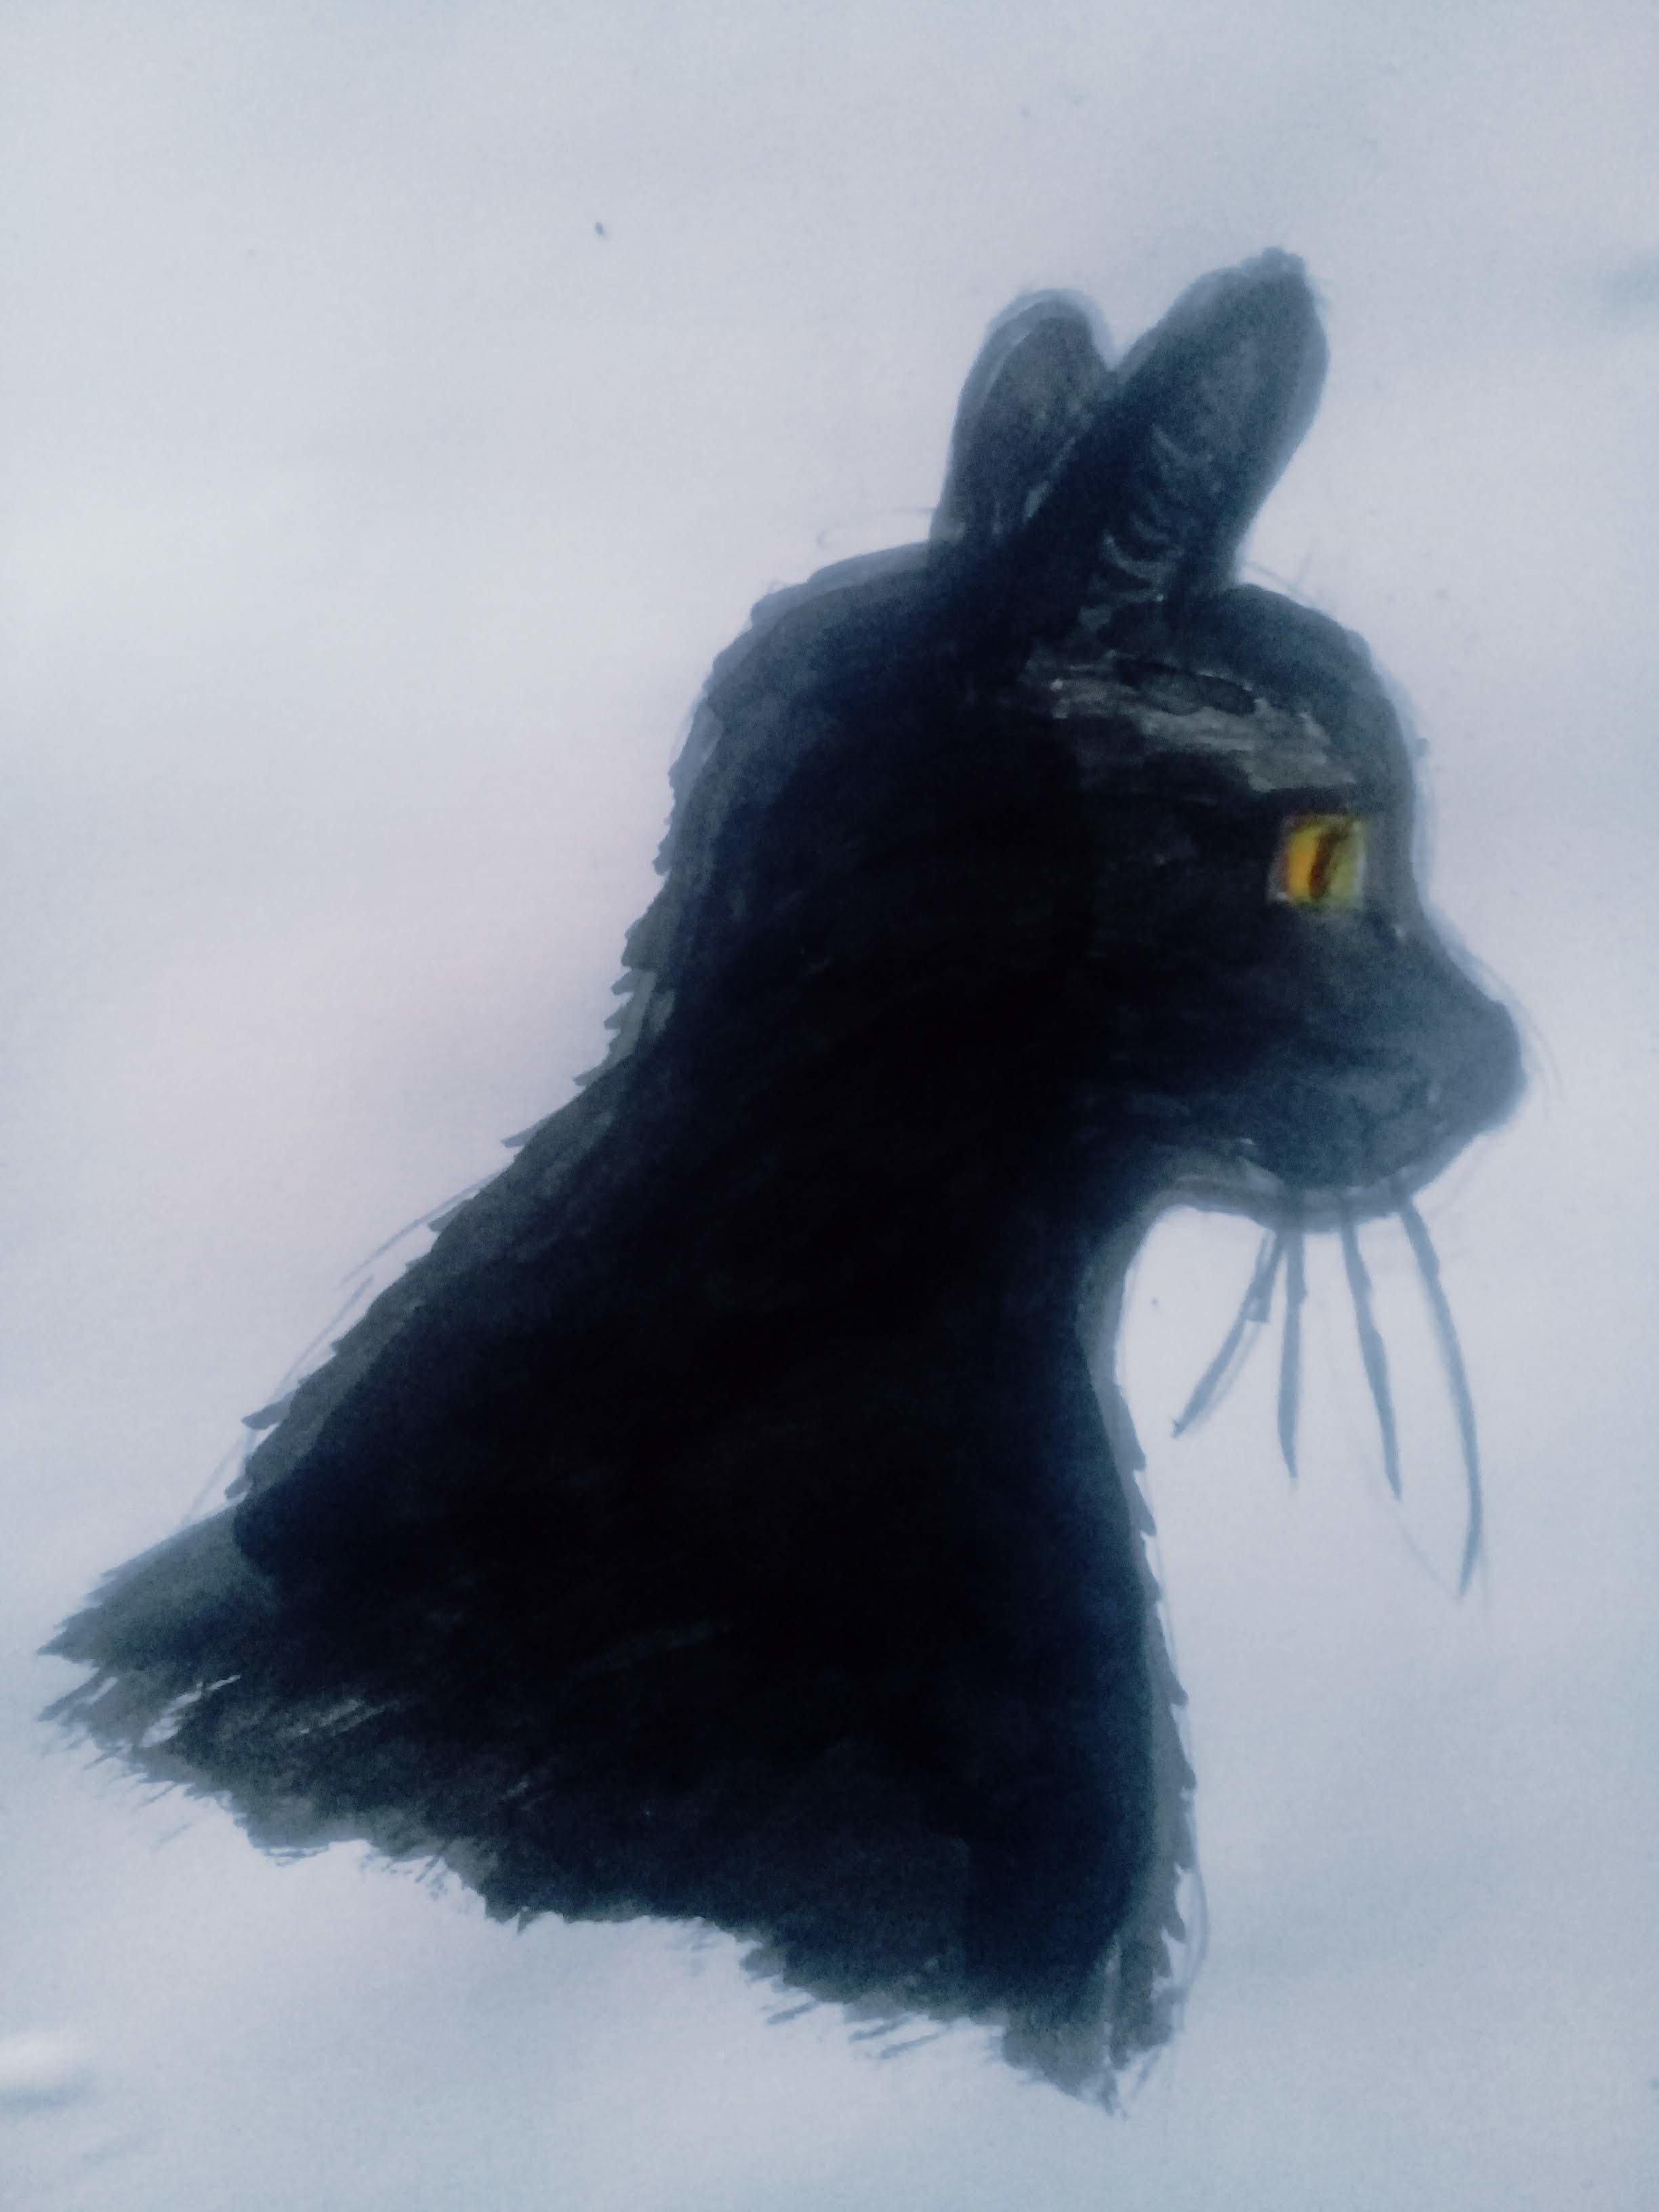
\includegraphics[height=\paperheight,angle=0]{retrato_cumple}};
	
	\node[text width=.5\textwidth,xshift=.25\textwidth,yshift=0cm,fill=white,draw=black] at (current page.center){ Y TAL VEZ NO LO RECUERDEN, PERO HACE UN AÑO, NACÍA YO EN CIUDADELA, NO MUY LEJOS DE CASA. MI MADRE ERA UNA GATA NARANJA ATIGRADA.
		
		TUVE TRES HERMANOS Y UNA HERMANA. DOS DE ELLOS ERAN NEGRITOS COMO YO Y MI HERMANA Y EL OTRO HERMANITO ERAS NARANJAS.
		
		ME ADOPTARON EL DÍA DE LA PRIMAVERA Y FUE ENTONCES QUE CONOCÍ MI NUEVA CASA DONDE SOY MUY FELIZ.
		
		ASI QUE ¡¡HOY ES MI CUMPLE!!};
	
	\node[xshift=-.3\textwidth,yshift=-.5\textheight,fill=white,draw=black,scale=1.3] at (current page.center){ 15 DE AGOSTO.};
\end{tikzpicture}
\newpage
\begin{tikzpicture}[remember picture, overlay]
	\node [inner sep=0pt, minimum width=\paperwidth, minimum height=\paperheight,opacity=1] at (current page.center) {
\includegraphics[width=\paperwidth,height=\paperheight,angle=0]{paper17.png}};
	
\end{tikzpicture}
TAMBIÉN EL 15 DE AGOSTO, PERO DE 1944, NACIÓ MI ABUELO HUMANO. ÉL VIVIÓ EN LA CASA DONDE HABITO CON MI PAPÁ ADOPTIVO. SE LLAMABA DANIEL, Y LE GUSTABAN TODO TIPO DE MASCOTAS, GATOS Y PERROS. TAMBIÉN LE GUSTABA PLANTAR ÁRBOLES, EL ÁRBOL POR DONDE PUDE SALIR DE LA CASA, EL TILO, LO HABÍA PLANTADO EL ABUELO HACÍA MÁS DE 10 AÑOS.

LAS GRANDES BIBLIOTECAS QUE HAY EN LA CASA, ALGUNA VEZ FUERON SUYAS. LEÍA MUCHO, TODO TIPO DE LIBROS. COMO HABÍA PASADO UNA NIÑEZ DIFÍCIL, LE AGRADABA UN AUTOR LLAMADO CHARLES DICKENS, QUE ESCRIBIÓ VARIAS NOVELAS SOBRE HISTORIAS DE NIÑOS Y NIÑAS CON PROBLEMAS. MI PAPÁ HEREDÓ ESE CARIÑO POR DICKENS Y TIENE MÁS DE 10 LIBROS ESCRITOS POR ÉL. UNA DE SUS HISTORIAS FAVORITAS SE LLAMA OLIVER TWIST.




\newpage
\begin{tikzpicture}[remember picture, overlay]
	\node [inner sep=0pt, minimum width=\paperwidth, minimum height=\paperheight,opacity=1] at (current page.center) {
\includegraphics[width=\paperwidth,height=\paperheight,angle=0]{paper12.png}};
	\node [inner sep=0pt, minimum width=.5\paperwidth, minimum height=.8\paperheight,opacity=1,xshift=-.2\textwidth] at (current page.center) {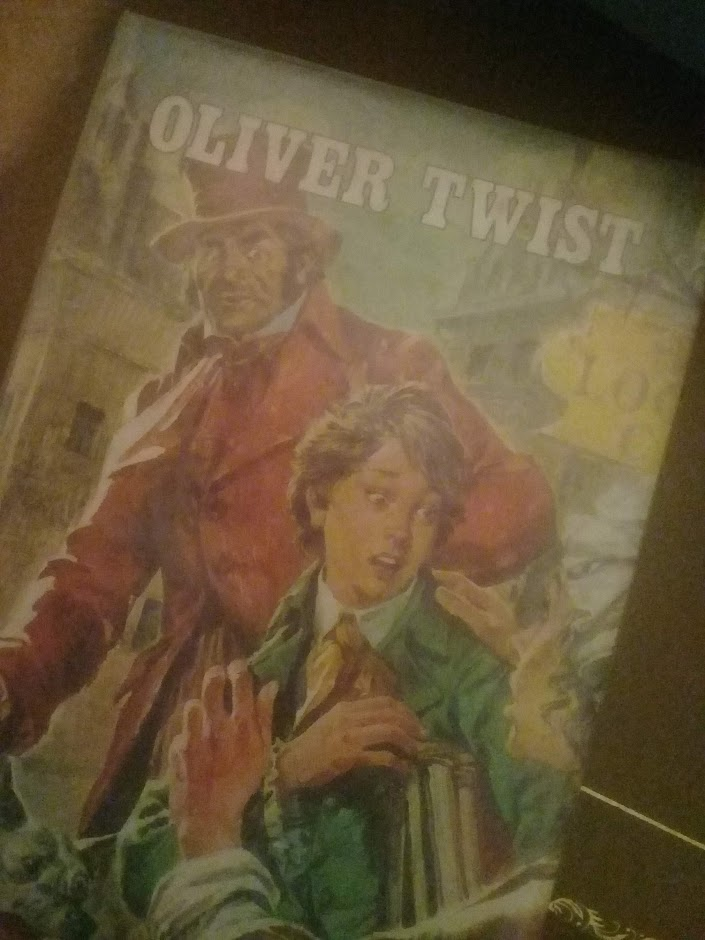
\includegraphics[width=.5\paperwidth]{oliver_twist}};
	\node[text width=.4\textwidth,xshift=.3\textwidth,yshift=0cm] at (current page.center){
		COMO VISITO MUCHO LAS BIBLIOTECAS CUANDO QUIERO DESCANSAR EN ALTURAS, PUDE VER EL LIBRO DE OLIVER. 
		
		PARECE UN JOVENCITO ALGO ASUSTADO. Y AHORA QUE CONOZCO LA HISTORIA, YA LO CREO QUE ESTARÍA ASUSTADO, DETRÁS SUYO ESTÁ BILL SIKES, UN SEÑOR MUY MALVADO ACOMPAÑADO DE UN PERRO INTIMIDANTE.
		
	};
\end{tikzpicture}
\newpage
\begin{tikzpicture}[remember picture, overlay]
	\node [inner sep=0pt, minimum width=\paperwidth, minimum height=\paperheight,opacity=1] at (current page.center) {
\includegraphics[width=\paperwidth,height=\paperheight,angle=0]{paper9.png}};
\end{tikzpicture}
-¿Y POR QUÉ ME GUSTARÍA A MÍ, UN FELINO DOMÉSTICO, LA HISTORIA DE OLIVER? ¿PORQUE ENCONTRÉ A UN SEÑOR CON UN PERRO TEMIBLES QUE ME CORRIERON Y CASI ME MOJAN? 
NO, NO ES SÓLO ESO. PUES OLIVER, COMO YO, FUE ADOPTADO Y PUDO CONOCER TAMBIÉN EL AFECTO EN AMIGOS, AMIGAS Y EN UNA FAMILIA. TUVO AVENTURAS EMOCIONANTES, POR MOMENTOS HASTA PENSÉ QUE NUNCA IBA A PODER REGRESAR Y ¡DABA HASTA ALGO DE MIEDO! 

UNA VERSIÓN ANIMADA SE HIZO EN 1989, Y NO PUDE DEJAR DE VERLA PUES, EN ESA PELÍCULA, ¡EL PROTAGONISTA OLIVER ES UN PEQUEÑO GATO!
LA HISTORIA ES MUY BUENA EN ESA VERSIÓN, PERO EN EL LIBRO PODRÍAN DESCUBRIR MUCHAS MÁS COSAS, POR EJEMPLO: ¿QUE PASABA CON ALGUNOS NIÑOS HACE DOSCIENTOS AÑOS?
OJALÁ ALGÚN DÍA LA LEAN, OLIVER SUPO INSPIRAR AMOR EN MUCHAS BUENAS PERSONAS Y SUPERAR LOS TIEMPOS MÁS DIFÍCILES.



\newpage
\begin{tikzpicture}[remember picture, overlay]
	\node [inner sep=0pt, minimum width=\paperwidth, minimum height=\paperheight,opacity=1] at (current page.center) {
\includegraphics[width=\paperwidth,height=\paperheight,angle=0]{paper17.png}};
	
	\node [xshift=0cm,inner sep=0pt, minimum width=\paperwidth, minimum height=\paperheight,opacity=1] at (current page.center) {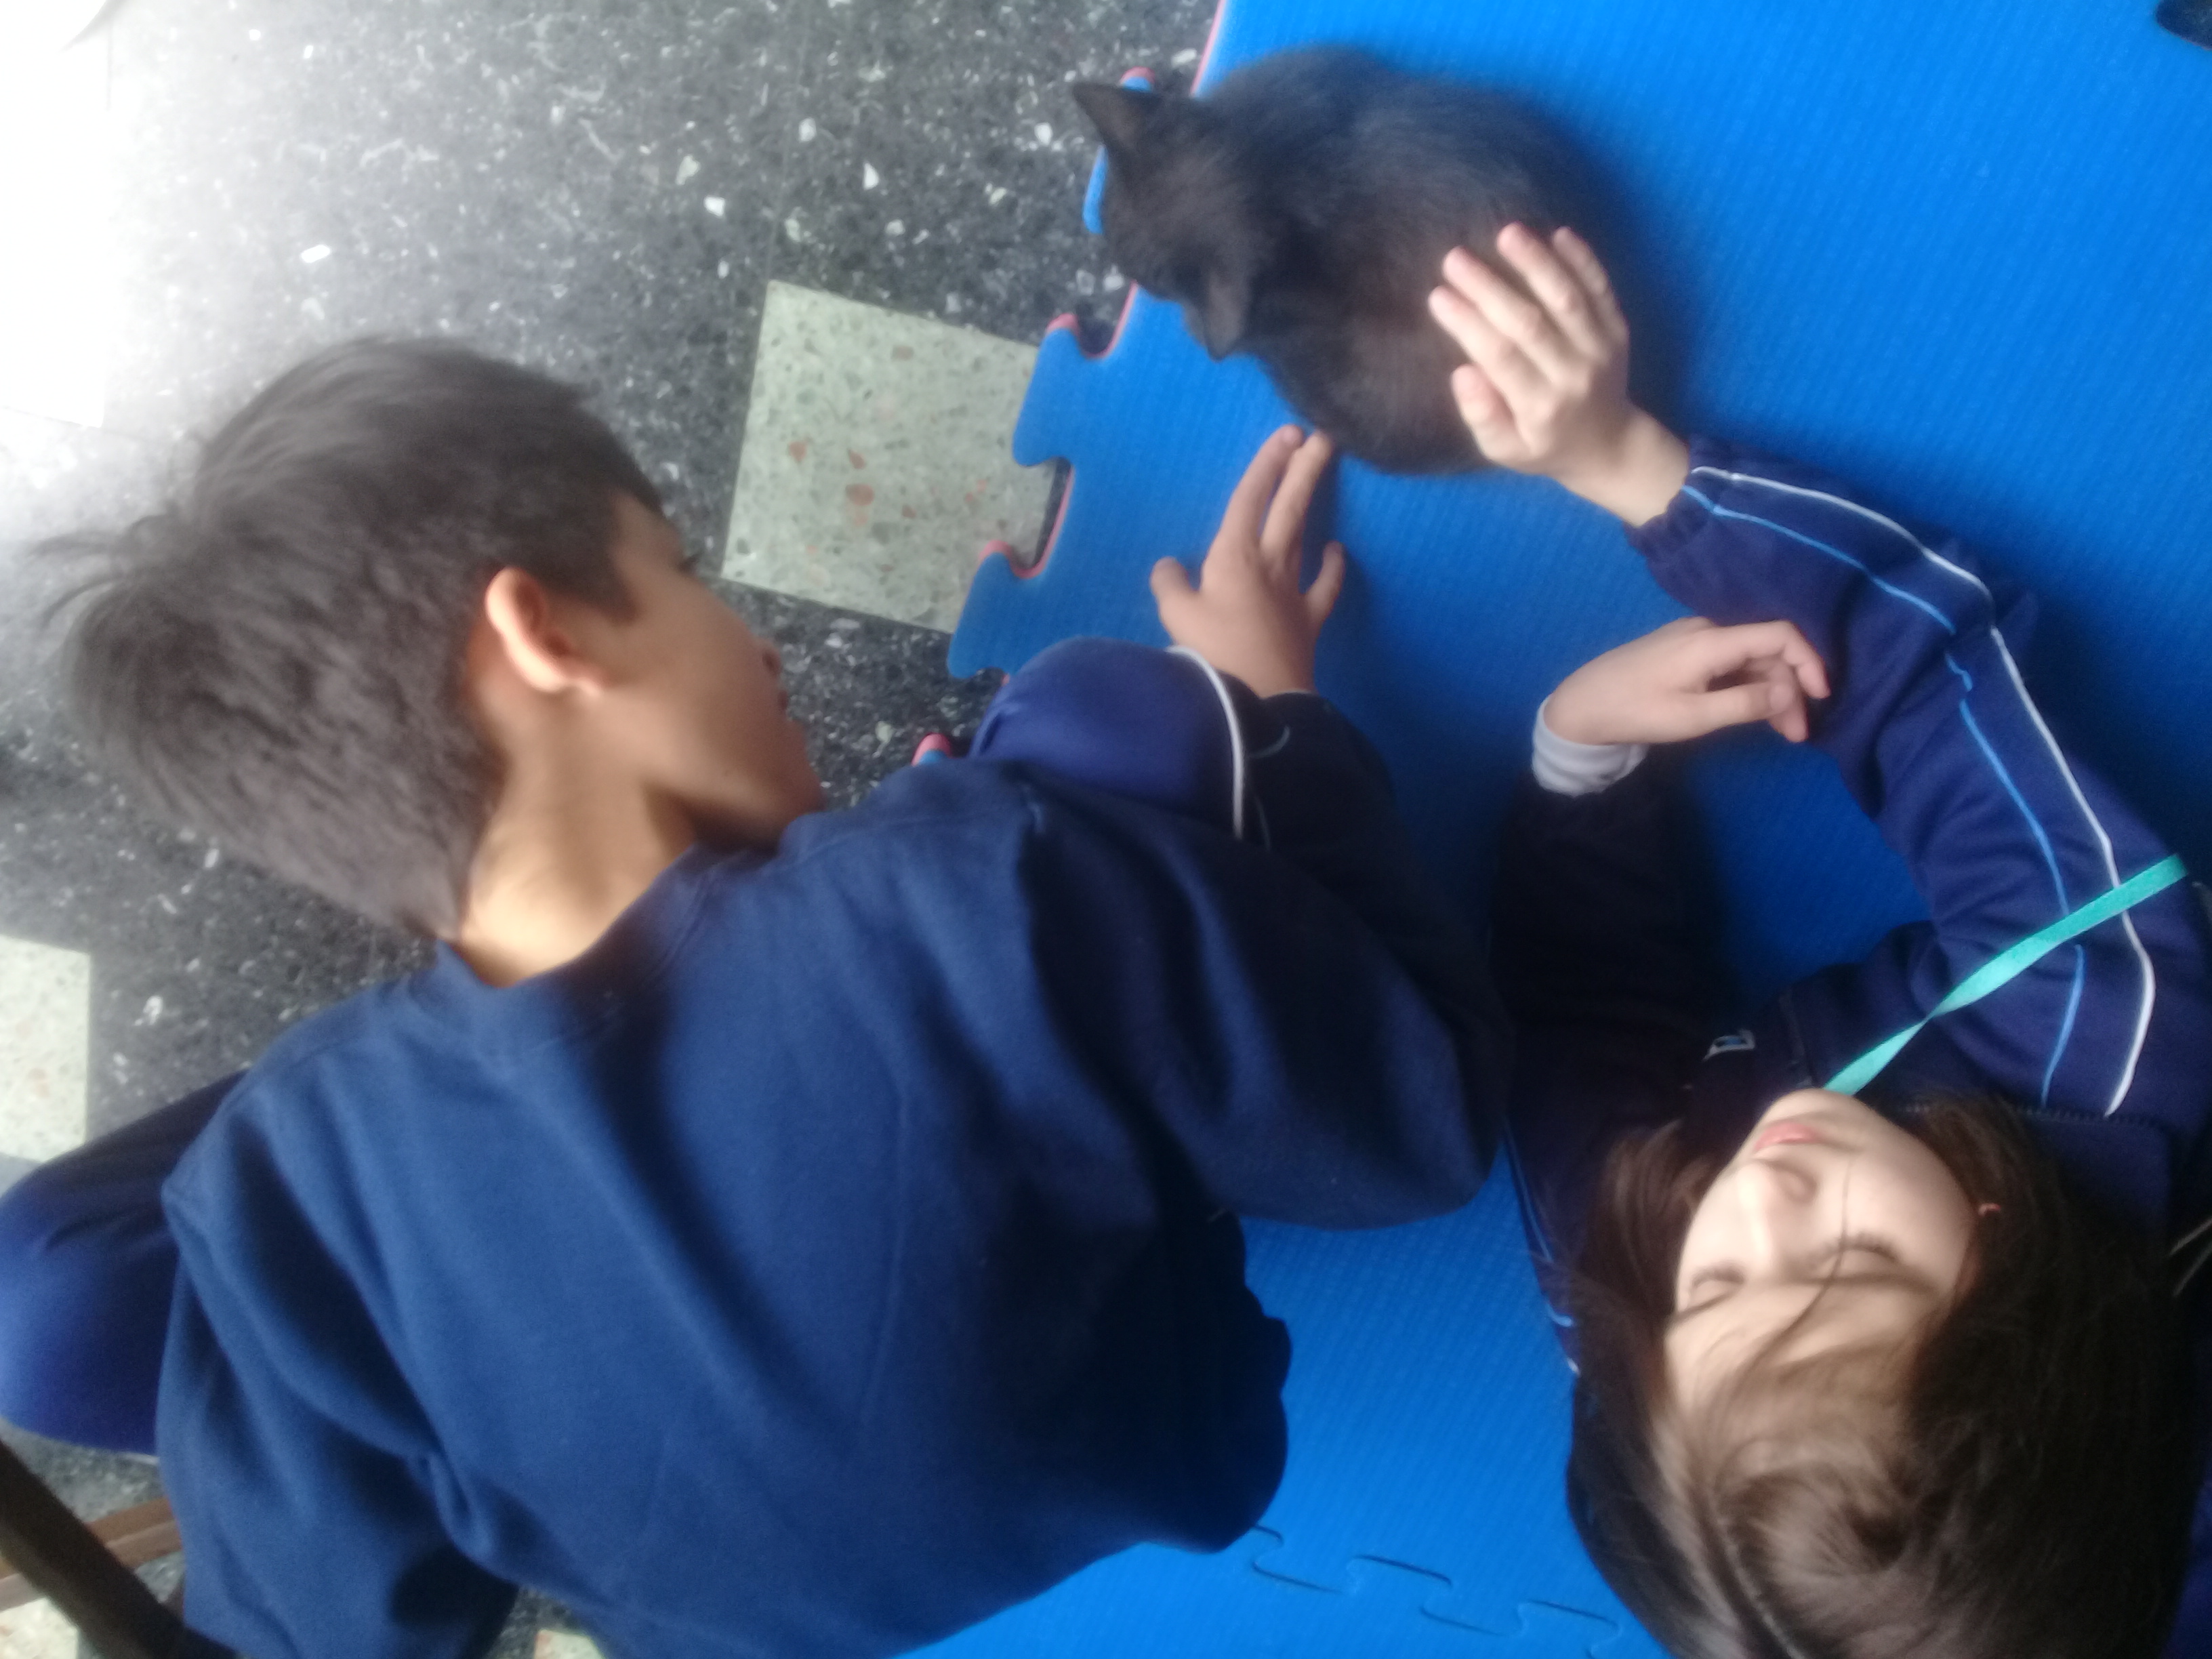
\includegraphics[height=.9\paperheight,angle=180]{hermanos}};
	\node[text width=.6\textwidth,xshift=.3\textwidth,yshift=-.42\textheight,fill=white,draw=black,scale=0.8] at (current page.center){ Y EN MI CASA FUI ASÍ RECIBIDO POR  MIS HERMANOS MAYORES HUMANOS: EDMOND Y A JEANNE, JUEGOS Y CARIÑO POR SIEMPRE.};
	
\end{tikzpicture}
\newpage
\begin{tikzpicture}[remember picture, overlay]
	\node [inner sep=0pt, minimum width=\paperwidth, minimum height=\paperheight,opacity=1] at (current page.center) {
\includegraphics[width=\paperwidth,height=\paperheight,angle=0]{paper9.png}};
\end{tikzpicture}
HOY ES EL DÍA DEL NIÑO Y TAMBIÉN DE LA NIÑA.

MIS QUERIDOS EDMOND Y JEANNE, DESEO QUE PRONTO PODAMOS VOLVERNOS A VER, NOS AGUARDAN DÍAS MUY FELICES PARA SEGUIR DISFRUTANDO LA NIÑEZ. DESCUBRIR JUNTOS LUGARES, GUSTOS Y PERFUMES DE VIEJOS Y NUEVOS MUNDOS.

Y POR SUPUESTO, ¡MUCHAS MÁS AVENTURAS JUNTOS CON OTTOKO!

LOS AMAMOS.



\newpage
\begin{tikzpicture}[remember picture, overlay]
	\node [inner sep=0pt, minimum width=\paperwidth, minimum height=\paperheight,opacity=1] at (current page.center) {
\includegraphics[width=\paperwidth,height=\paperheight,angle=0]{paper17.png}};
	
	\node [xshift=0cm,inner sep=0pt, minimum width=\paperwidth, minimum height=\paperheight,opacity=1] at (current page.center) {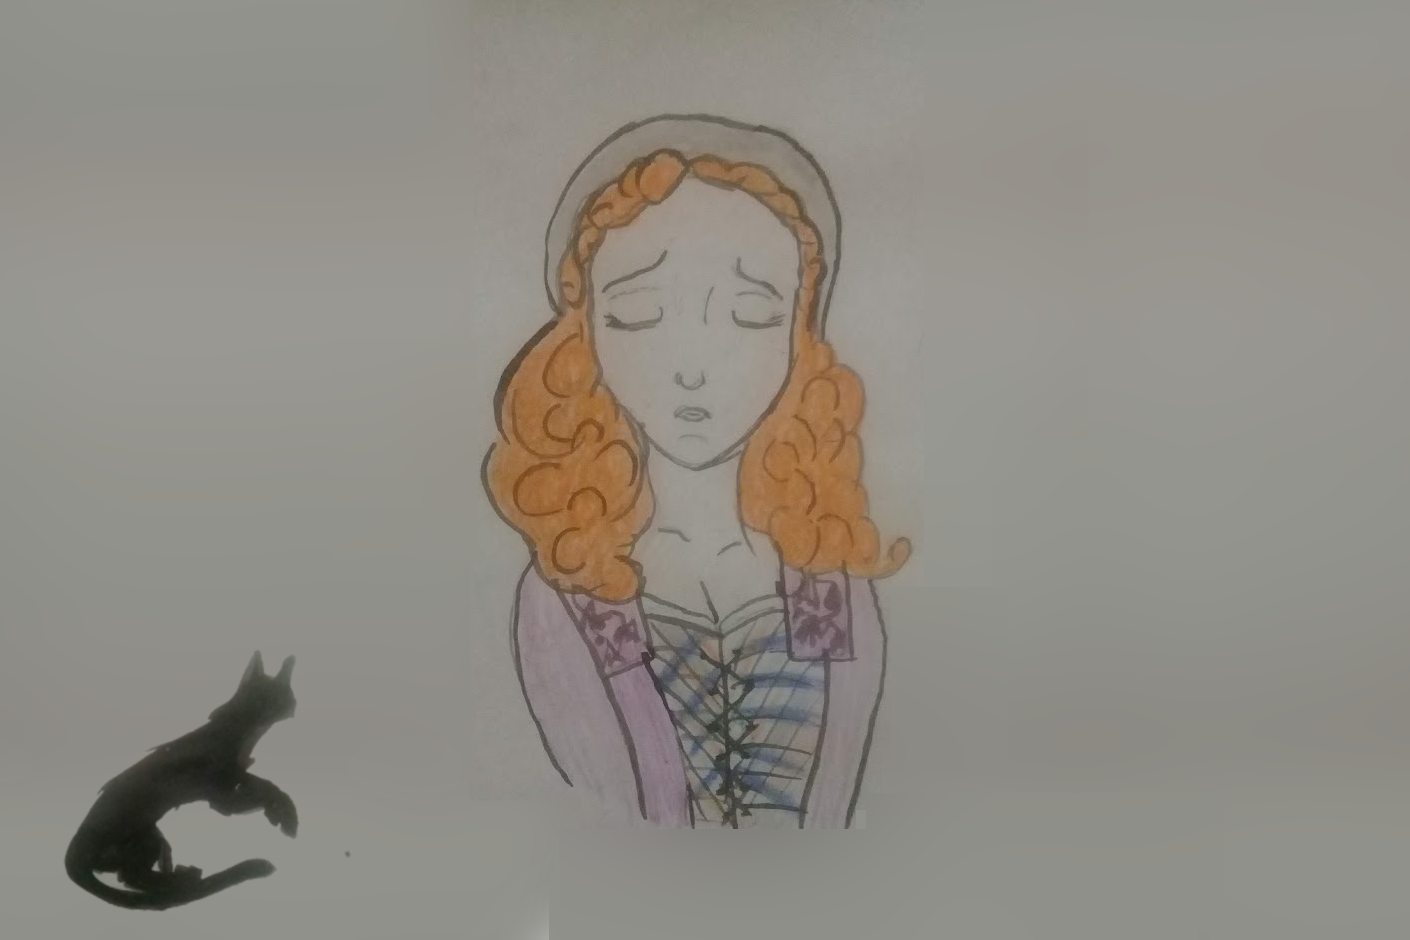
\includegraphics[height=\paperheight,angle=0]{nancy}};
	
	
\end{tikzpicture}

\newpage
\begin{tikzpicture}[remember picture, overlay]
	\node [inner sep=0pt, minimum width=\paperwidth, minimum height=\paperheight,opacity=1] at (current page.center) {
\includegraphics[width=\paperwidth,height=\paperheight,angle=0]{paper7.png}};
	
\end{tikzpicture}
NO QUERÍA DEJAR DE COMPARTIRLES LA IMAGEN QUE ME HICE DE NANCY. ME GUSTA, ANTES DE DORMIR, PENSAR UN RATO EN LAS AVENTURAS VIVIDAS Y EN LAS LEÍDAS. YA AL BORDE DEL SUEÑO, EN AQUELLAS QUE ME ESPERAN Y ESCRIBIRÉ.

PODRÍAN PENSAR QUE NO HAY GRAN COSA EN LA CIUDAD QUE AGUARDE A UN HUMILDE GATO NEGRO. QUE NADA YA PUEDE SORPRENDER AL LADO DE LAS COLORIDAS Y LUMINOSAS ATRACCIONES QUE VEMOS EN LAS PANTALLAS. QUE TODA LA REALIDAD, TARDE O TEMPRANO, TERMINARÁ FORMANDO PARTE DE UN VIDEO QUE CONTENDRÁ APENAS ALGUNOS SEGUNDOS INTERESANTES.

PERO LOS GATOS SOMOS MUY PACIENTES Y CADA SEGUNDO, AÚN CUANDO ESTAMOS AL ACECHO SIN MOVERNOS, LO DISFRUTAMOS MUCHO.




\newpage
\begin{tikzpicture}[remember picture, overlay]
	\node [inner sep=0pt, minimum width=\paperwidth, minimum height=\paperheight,opacity=1] at (current page.center) {
\includegraphics[width=\paperwidth,height=\paperheight,angle=0]{paper7.png}};
	
\end{tikzpicture} 
SI OBSERVAN CON ATENCIÓN, EN MUCHAS DE LAS CALLES DE NUESTRA CIUDAD, HAY CÁMARAS DE VIDEO QUE GRABAN A TODA HORA, ALGUNAS CON UNA SENSIBILIDAD TAN GRANDE QUE NO NECESITAN QUE HAYA UNA BUENA ILUMINACIÓN. UN POCO COMO NUESTROS OJOS GATUNOS, QUE SON MUY BUENOS PARA VER CON POCA O MUCHA LUZ. 

PERO ESTE MUNDO DE VIDEOS NO ES LO QUE NOS GUSTA A LOS GATOS NEGROS, QUE BUSCAMOS LA INTIMIDAD, EL MISTERIO Y EL SECRETO DE NUESTRAS INTENCIONES, GESTOS Y MOVIMIENTOS. ¡QUÉ CLASE DE CAZADORES SERÍAMOS SIN ELLO!
CADA DÍA BUSCO LOS ESPACIOS OSCUROS PARA OCULTARME, PARA PODER SORPRENDER A MI PADRE CON ALGÚN DESPREVENIDO ZARPAZO. ME IMAGINO QUE DEBE ESTAR MUY ORGULLOSO CADA VEZ QUE CONSIGO SOBRESALTARLO, PUES ME ELOGIA A LOS GRITOS. TODAS ESAS COSAS PENSABA ANTES DE DORMIR Y JUSTO DESPUÉS DE LEVANTARME POR LA MAÑANA.


\newpage
\begin{tikzpicture}[remember picture, overlay]
	\node [inner sep=0pt, minimum width=\paperwidth, minimum height=\paperheight,opacity=1] at (current page.center) {
\includegraphics[width=\paperwidth,height=\paperheight,angle=0]{paper17.png}};
	
	\node [xshift=0cm,inner sep=0pt, minimum width=\paperwidth, minimum height=\paperheight,opacity=1] at (current page.center) {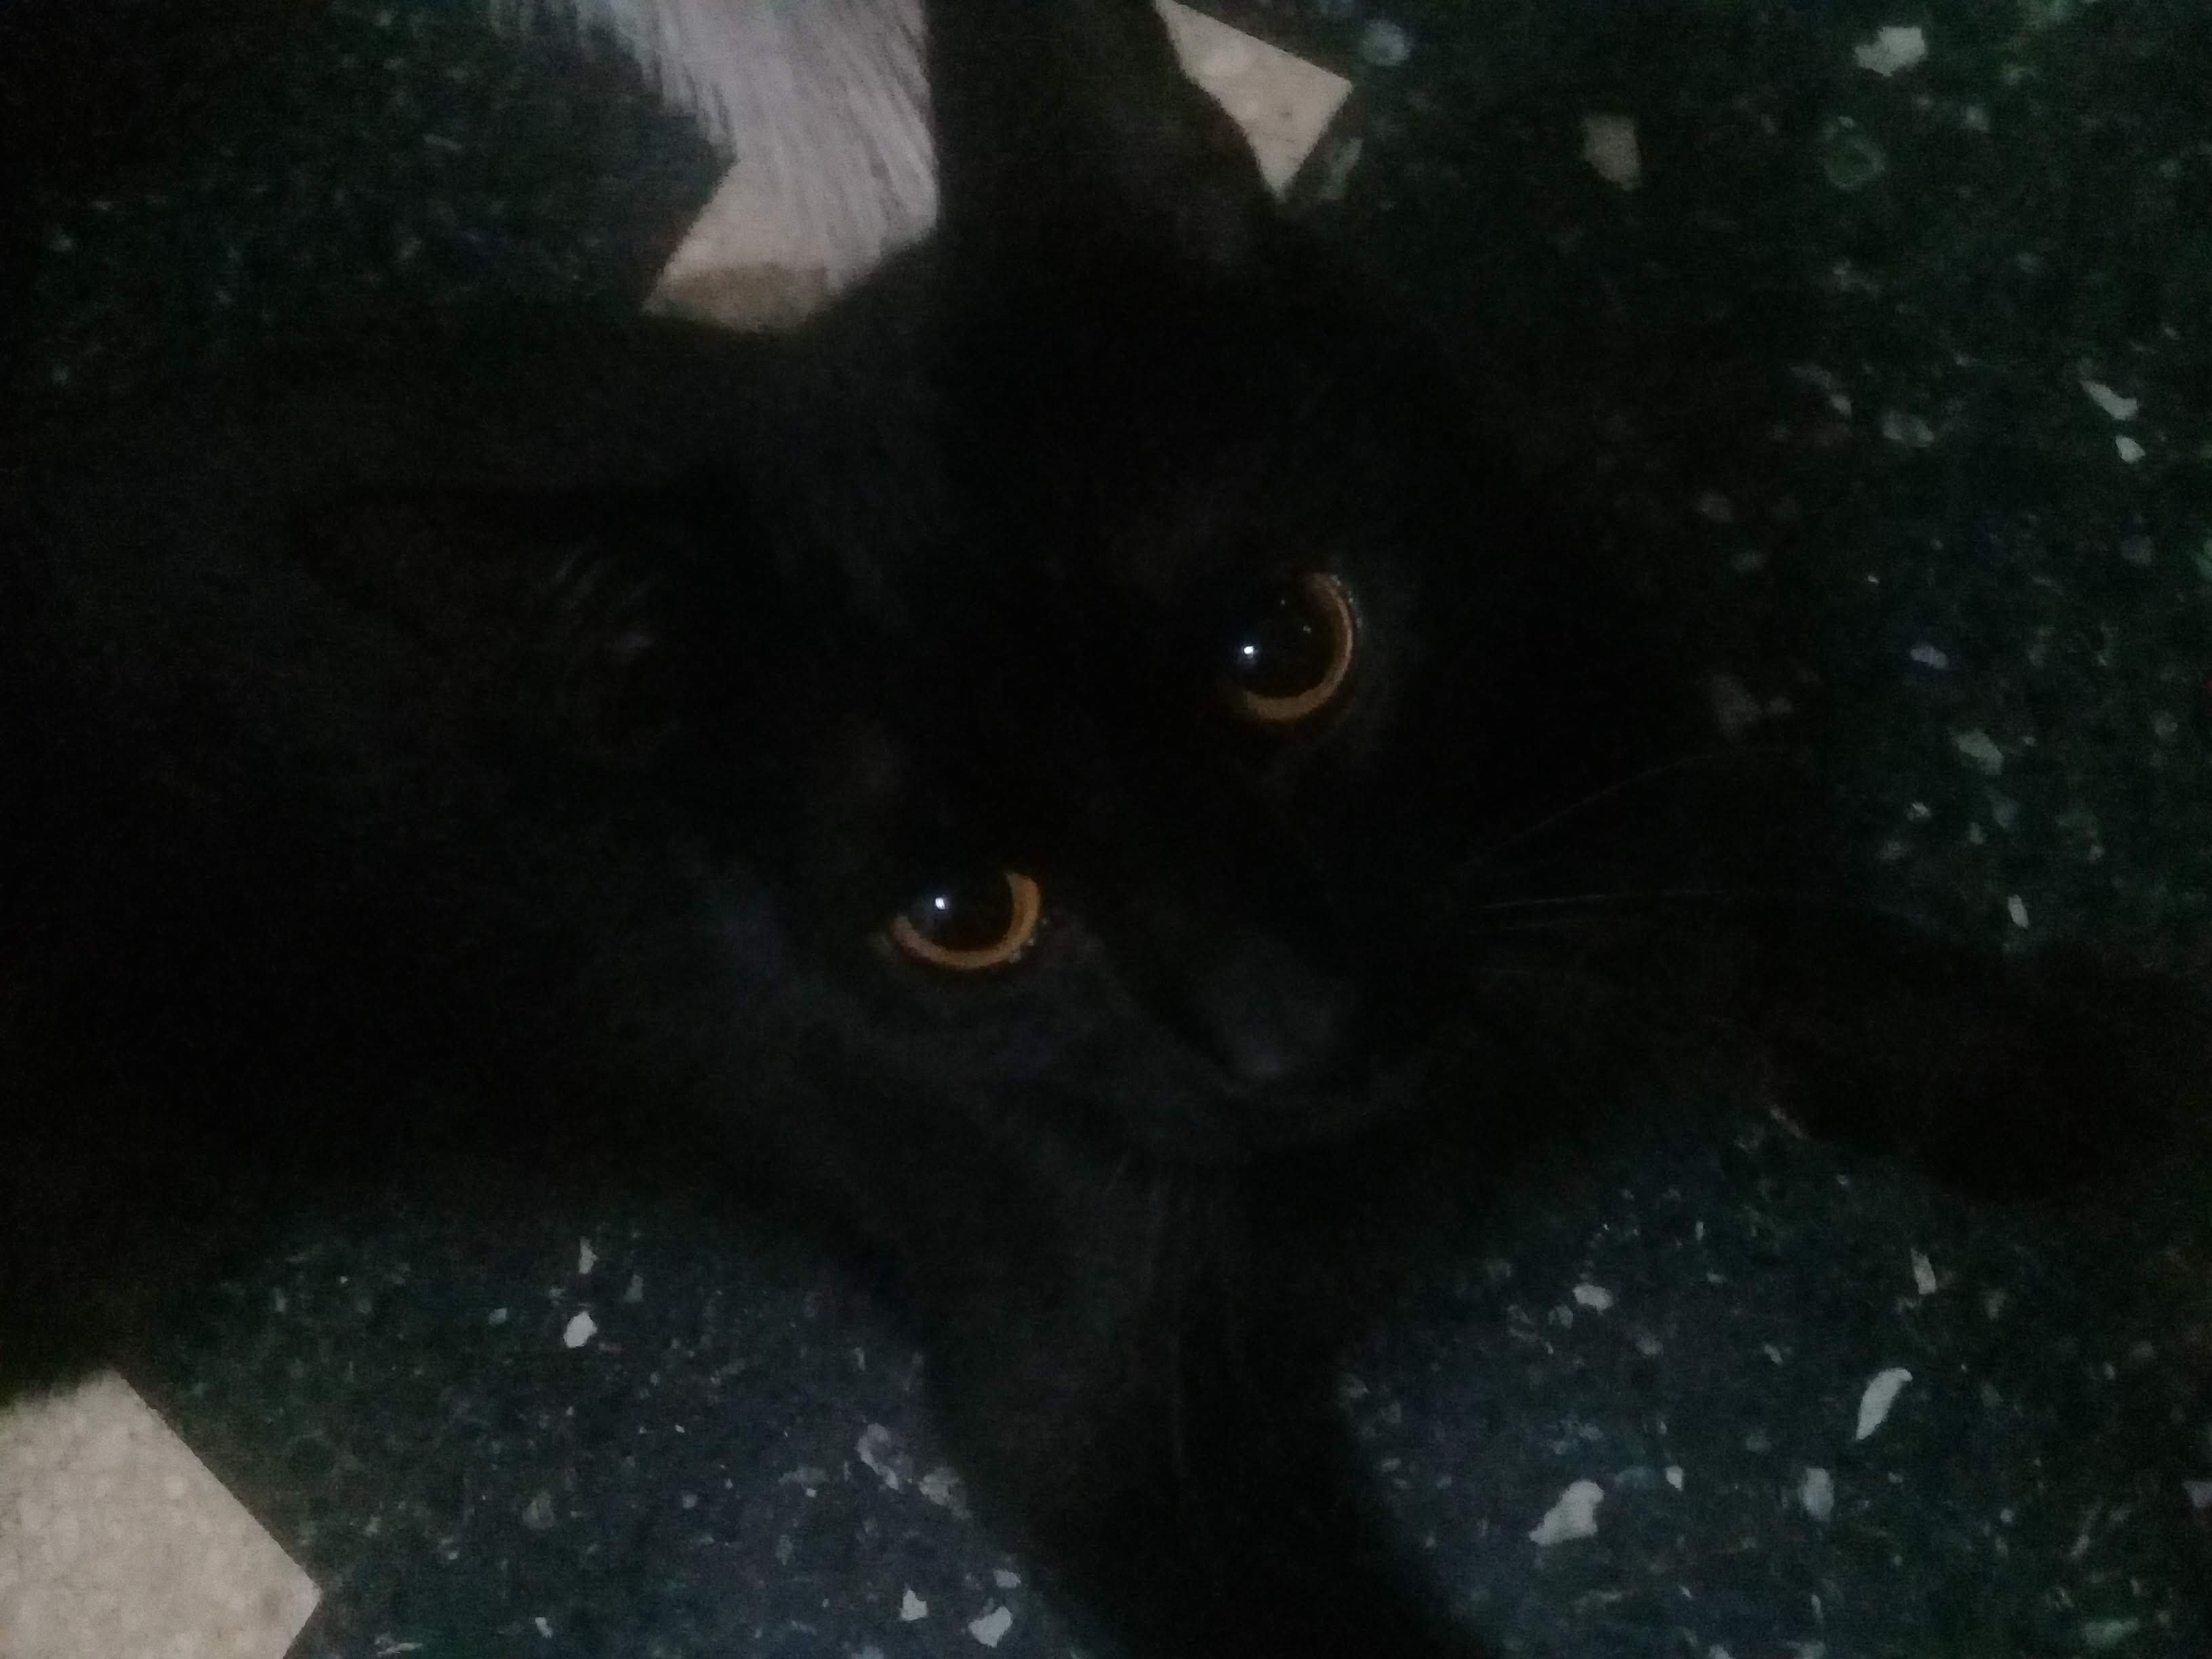
\includegraphics[width=.9\paperwidth,angle=0]{negrura}};
	
	
\end{tikzpicture}

\vspace{.8\textheight}
\textcolor{yellow}{LOS GATOS NEGROS PREFERIMOS LOS LUGARES OSCUROS.}		

\newpage
\begin{tikzpicture}[remember picture, overlay]
	\node [inner sep=0pt, minimum width=\paperwidth, minimum height=\paperheight,opacity=1] at (current page.center) {
\includegraphics[width=\paperwidth,height=\paperheight,angle=0]{paper17.png}};
\end{tikzpicture}
LOS DÍAS SE VUELVEN MÁS CÁLIDOS, EL SOL SE FILTRA POR MI CASA POR MÁS TIEMPO Y CON MÁS FUERZA. AFUERA LAS PLANTAS TIENEN MUCHAS HOJAS QUE BROTARON Y CRECEN CON FUERZA. AÚN AQUELLAS QUE PENSÁBAMOS QUE HABÍAN ACABADO.

UNA PLANTA ESPECIAL GUARDA MI PAPÁ Y TRATA DE CUIDAR CON PACIENCIA. CRECIÓ DESDE UNA SEMILLA, PASANDO TRES MESES ENVUELTA EN PAPEL DENTRO DE LA HELADERA. HABÍA MUCHAS SEMILLAS, Y EMPEZARON A GERMINAR, ASÍ PARECE QUE SE LE DICE EN LAS CIENCIAS NATURALES, EN SEPTIEMBRE DEL AÑO PASADO. ¡JUSTO ANTES DE QUE ME ADOPTARAN!

PODRÍA QUE PENSAR QUE ESA PLANTA ES UNA ESPECIE DE HERMANA DEL MUNDO VEGETAL.





\newpage
\begin{tikzpicture}[remember picture, overlay]
	\node [inner sep=0pt, minimum width=\paperwidth, minimum height=\paperheight,opacity=1] at (current page.center) {
\includegraphics[width=\paperwidth,height=\paperheight,angle=0]{paper17.png}};
\end{tikzpicture}
\begin{normalsize}
	
	ALGÚN DÍA, SUEÑA MI PAPÁ, ESA PLANTA CRECERÁ Y SERÁ UN ÁRBOL PRECIOSO. SI BIEN SE LE LLAMA CEREZO, NO DA FRUTAS SINO UNAS FLORES DE COLOR ROSA. NO ES UNA ESPECIE NATIVA SINO QUE VIENE DE MUY LEJOS, DEL JAPÓN, UN PAÍS QUE ESTÁ EN LAS ANTÍPODAS DEL NUESTRO. ES DECIR, SI CON MIS GARRITAS EMPEZARÁ YO A CAVAR UN POZO, ATRAVESANDO TODO EL PLANETA, LLEGARÍA CERCA DE ALLÍ.  PUEDE  QUE EN EL MEDIO DEL TRAYECTO HABRÍA LAVA A ALTÍSIMAS TEMPERATURAS, CON UN POZO ASÍ ENTIENDO BIEN EL ASUNTO DE LAS ANTÍPODAS.
	
	EN NUESTRA CIUDAD, HAY MUCHOS ÁRBOLES DE SAKURA EN EL JARDÍN JAPONÉS. ESTÁ UN TANTO LEJOS DE NUESTRO BARRIO PERO SE PUEDE LLEGAR 
	
\end{normalsize}	



\newpage
\begin{tikzpicture}[remember picture, overlay]
	\node [inner sep=0pt, minimum width=\paperwidth, minimum height=\paperheight,opacity=1] at (current page.center) {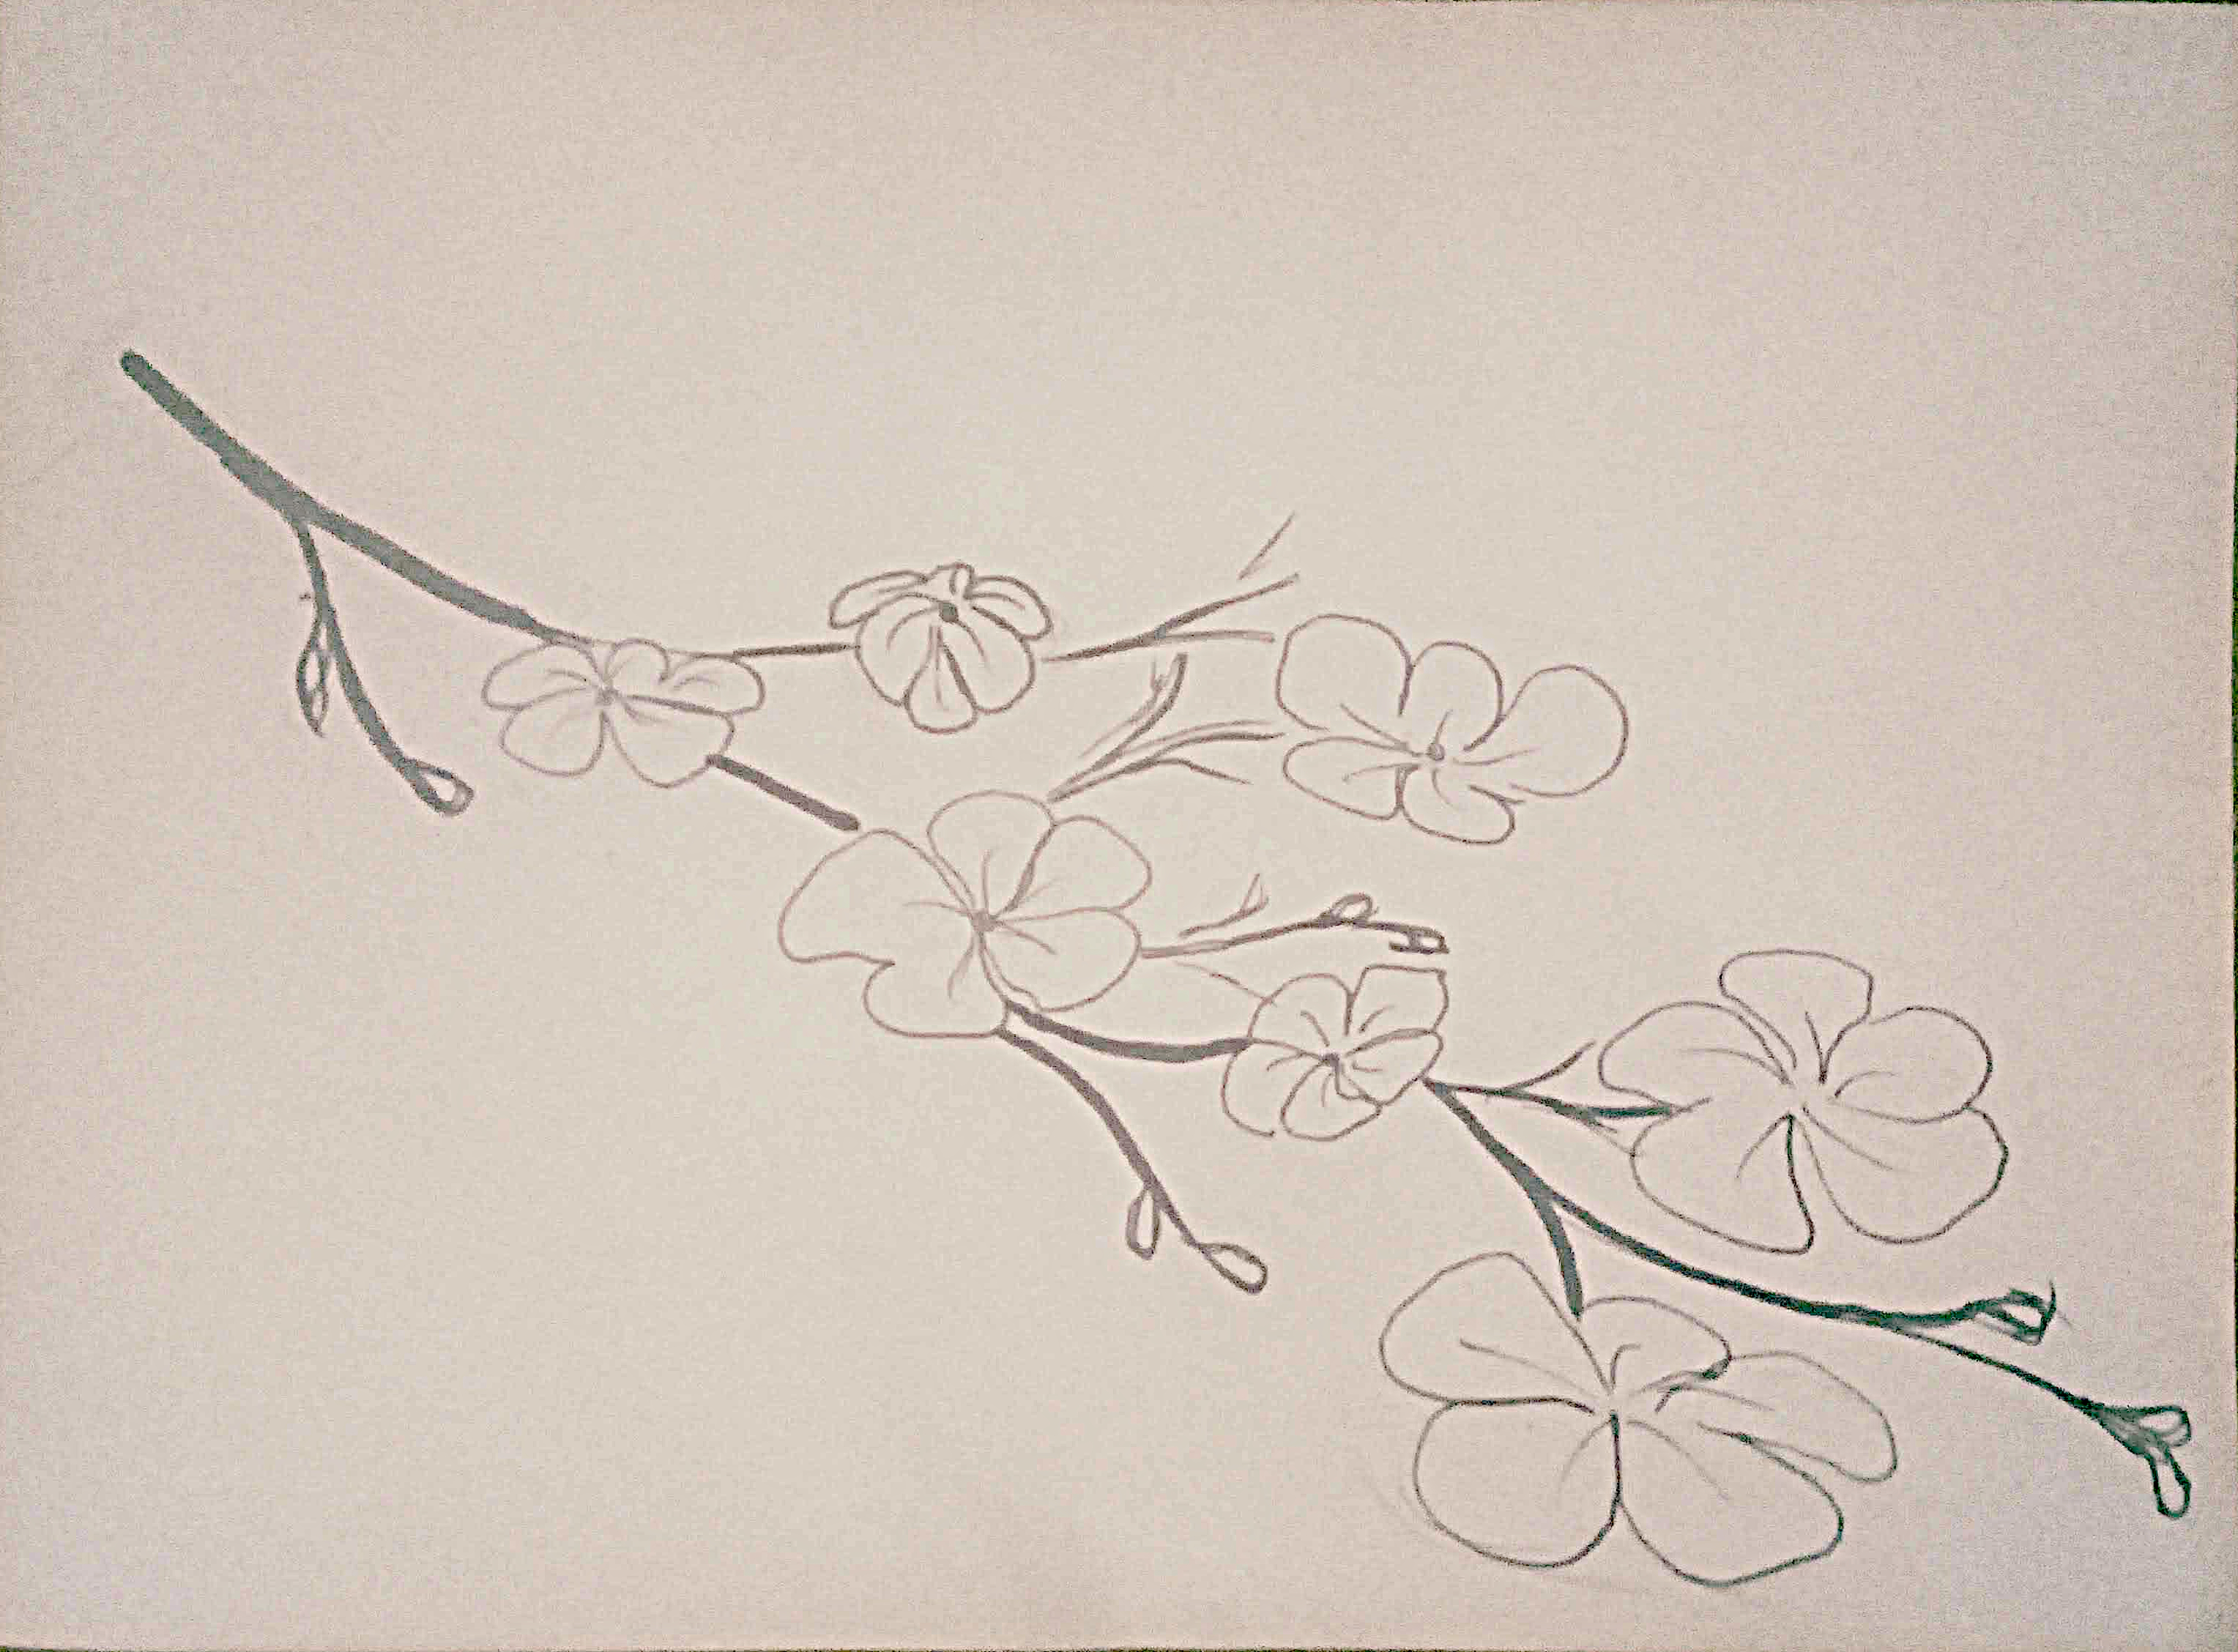
\includegraphics[width=\paperwidth,height=\paperheight,angle=0]{sakura1}};
	
	
	
	
\end{tikzpicture}
\newpage
\begin{tikzpicture}[remember picture, overlay]
	\node [inner sep=0pt, minimum width=\paperwidth, minimum height=\paperheight,opacity=1] at (current page.center) {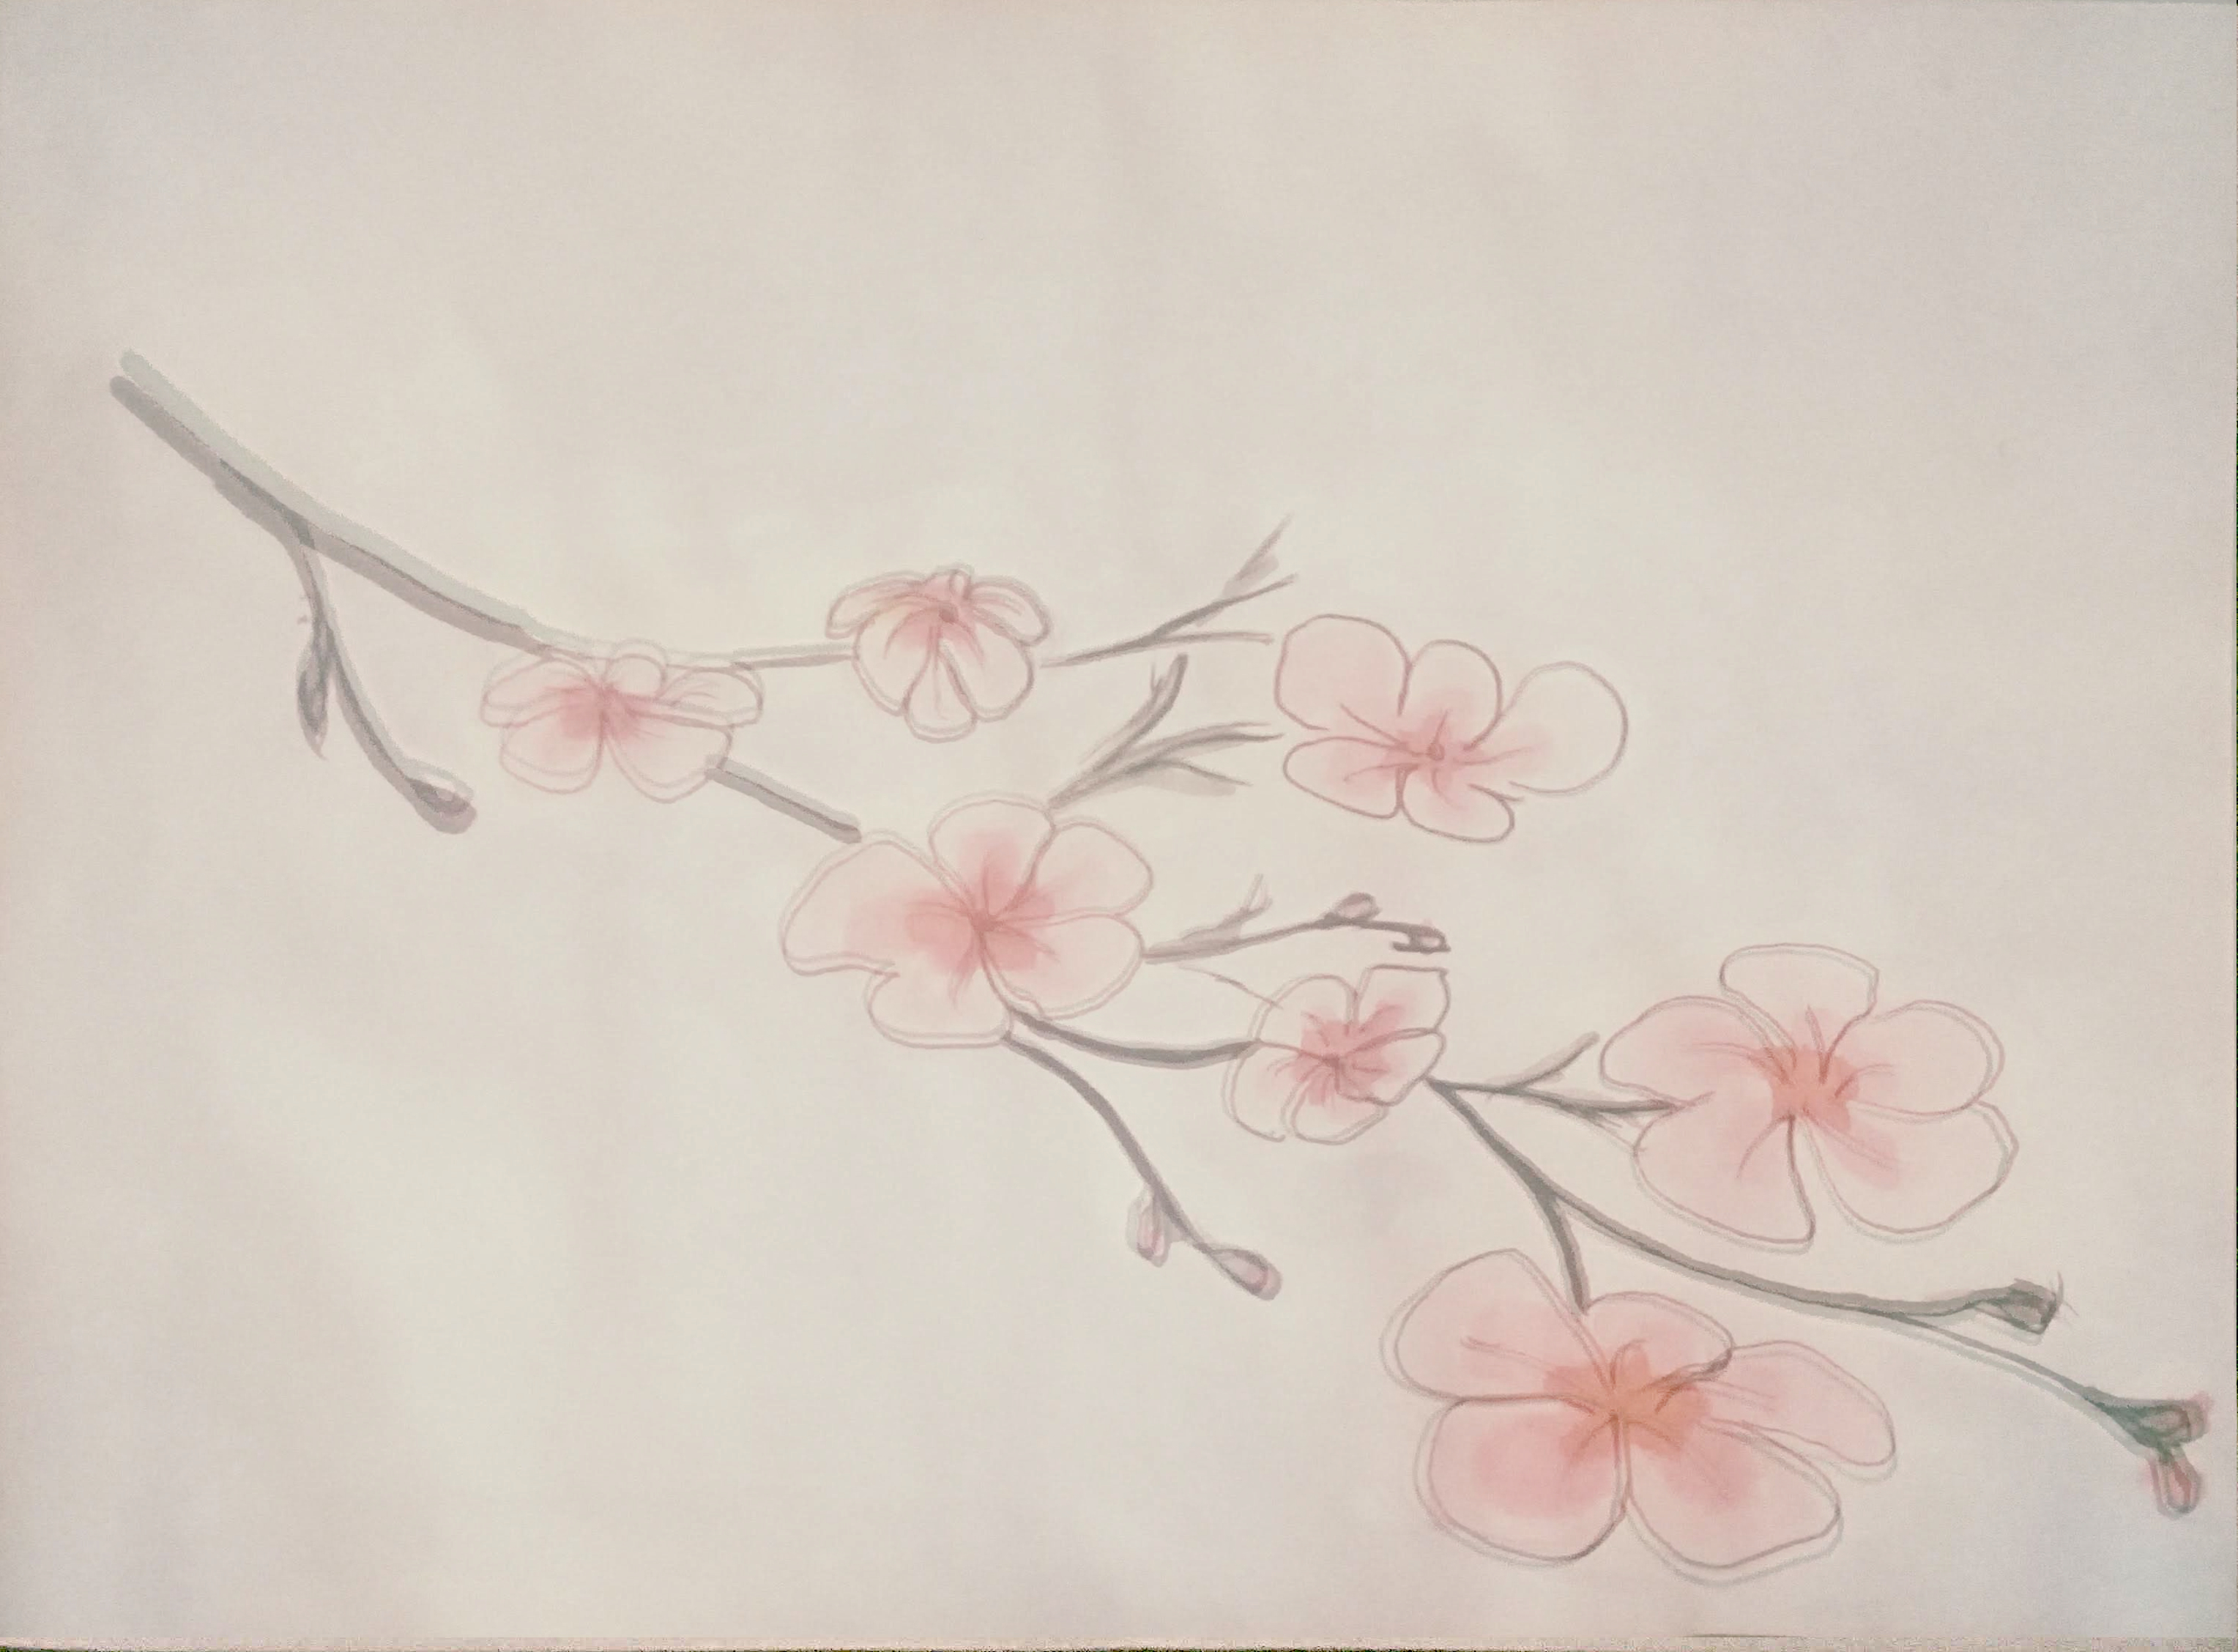
\includegraphics[width=\paperwidth,height=\paperheight,angle=0]{sakura2}};
	
\end{tikzpicture}
¡ESTAMOS EN LOS ÚLTIMOS DÍAS QUE SE PUEDEN APRECIAR LAS FLORES! SI NO LLEGAN A VERLAS, NO SE AFLIJAN, LAS SAKURA SON UN SÍMBOLO DE NUESTRA FRAGILIDAD Y DE QUE PODEMOS VOLVER A SER FELICES SI TENEMOS PACIENCIA.	



\newpage
\begin{tikzpicture}[remember picture, overlay]
	\node [inner sep=0pt, minimum width=\paperwidth, minimum height=\paperheight,opacity=1] at (current page.center) {
\includegraphics[width=\paperwidth,height=\paperheight,angle=0]{paper12.png}};
	
	
\end{tikzpicture}
EL SOL CADA MAÑANA SE LEVANTA MÁS CÁLIDO, ME PARECE QUE EN LA CALLE   LAS PERSONAS YA NO SE PONEN TANTAS CAPAS DE ROPA PARA ABRIGARSE. ¿VIERON EL  COLLAR CON CHAPITA		QUE LLEVO? ME LO PUSO MI PAPÁ, PARA QUE SI LLEGARA A SALIR OTRA VEZ DE LA CASA, LA GENTE SEPA MI NOMBRE Y EL TELÉFONO PARA DECIR DONDE ESTOY$\ldots$ ¡PERO YO NO PIENSO PERDERME, NO!

CON EL CALOR, EMPECÉ A NOTAR NUEVOS VISITANTES EN EL PATIO, O VIEJOS, PUES VUELVEN CADA AÑO. HACEN UN RUIDO MUY PARTICULAR, MÁS PRECISAMENTE SE LE DICE ZUMBIDO. LO HACEN PORQUE BATEN SUS ALAS A GRAN VELOCIDAD. A LAS PERSONAS SUELEN MOLESTARLES PERO PARA MÍ ES UNA NUEVA OPORTUNIDAD DE UNA BUENA CAZA. ¿SABEN DE QUE ANIMALES SE TRATA?




\newpage
\begin{tikzpicture}[remember picture, overlay]
	\node [inner sep=0pt, minimum width=\paperwidth, minimum height=\paperheight,opacity=1] at (current page.center) {
\includegraphics[width=\paperwidth,height=\paperheight,angle=0]{paper6}};
\end{tikzpicture}
LAS ABEJAS VIENEN AL PATIO CUANDO EMPIEZAN LOS DÍAS PRIMAVERALES PARA AYUDAR CON LA POLINIZACIÓN. ¡QUE PALABRA LARGA!

SE TRATA DE LO QUE OCURRE EN LAS PLANTAS PARA QUE A PARTIR DE UNA FLOR, SE PUEDAN PRODUCIR FRUTAS O SEMILLAS. LAS ABEJAS RECOLECTAN POLEN PARA LLEVARSELO A SU PANAL Y HACER MIEL.  POR ESO, DEPENDIENDO DE QUE FLORES FRECUENTAN LAS ABEJAS, CAMBIA EL GUSTO Y EL COLOR DE LA MIEL. ¿LES GUSTA A USTEDES LA MIEL? PARA UN GATO, ES UN GUSTO DEMASIADO AZUCARADO. 

DURANTE EL TRANSPORTE DE POLEN QUE HACEN LAS ABEJAS, PARTE CAE DONDE LUEGO SE FORMARÁN LAS FRUTAS Y ASÍ DE SU TRABAJO MUTUO SE BENEFICIAN ELLAS Y LAS PLANTAS.	

¿HAN VISTO QUE SOY UN GATO MUY INVESTIGADOR?
PERO, ¡ATENCIÓN! EN REALIDAD NO ME REFERÍA NECESARIAMENTE A LAS ABEJAS$\ldots$





\newpage
\begin{tikzpicture}[remember picture, overlay]
	\node [inner sep=0pt, minimum width=\paperwidth, minimum height=\paperheight,opacity=1] at (current page.center) {
\includegraphics[width=\paperwidth,height=\paperheight,angle=0]{paper6}};
	\node [xshift=.25\paperwidth,inner sep=0pt, minimum width=.5\paperwidth, minimum height=\paperheight,opacity=1] at (current page.center) {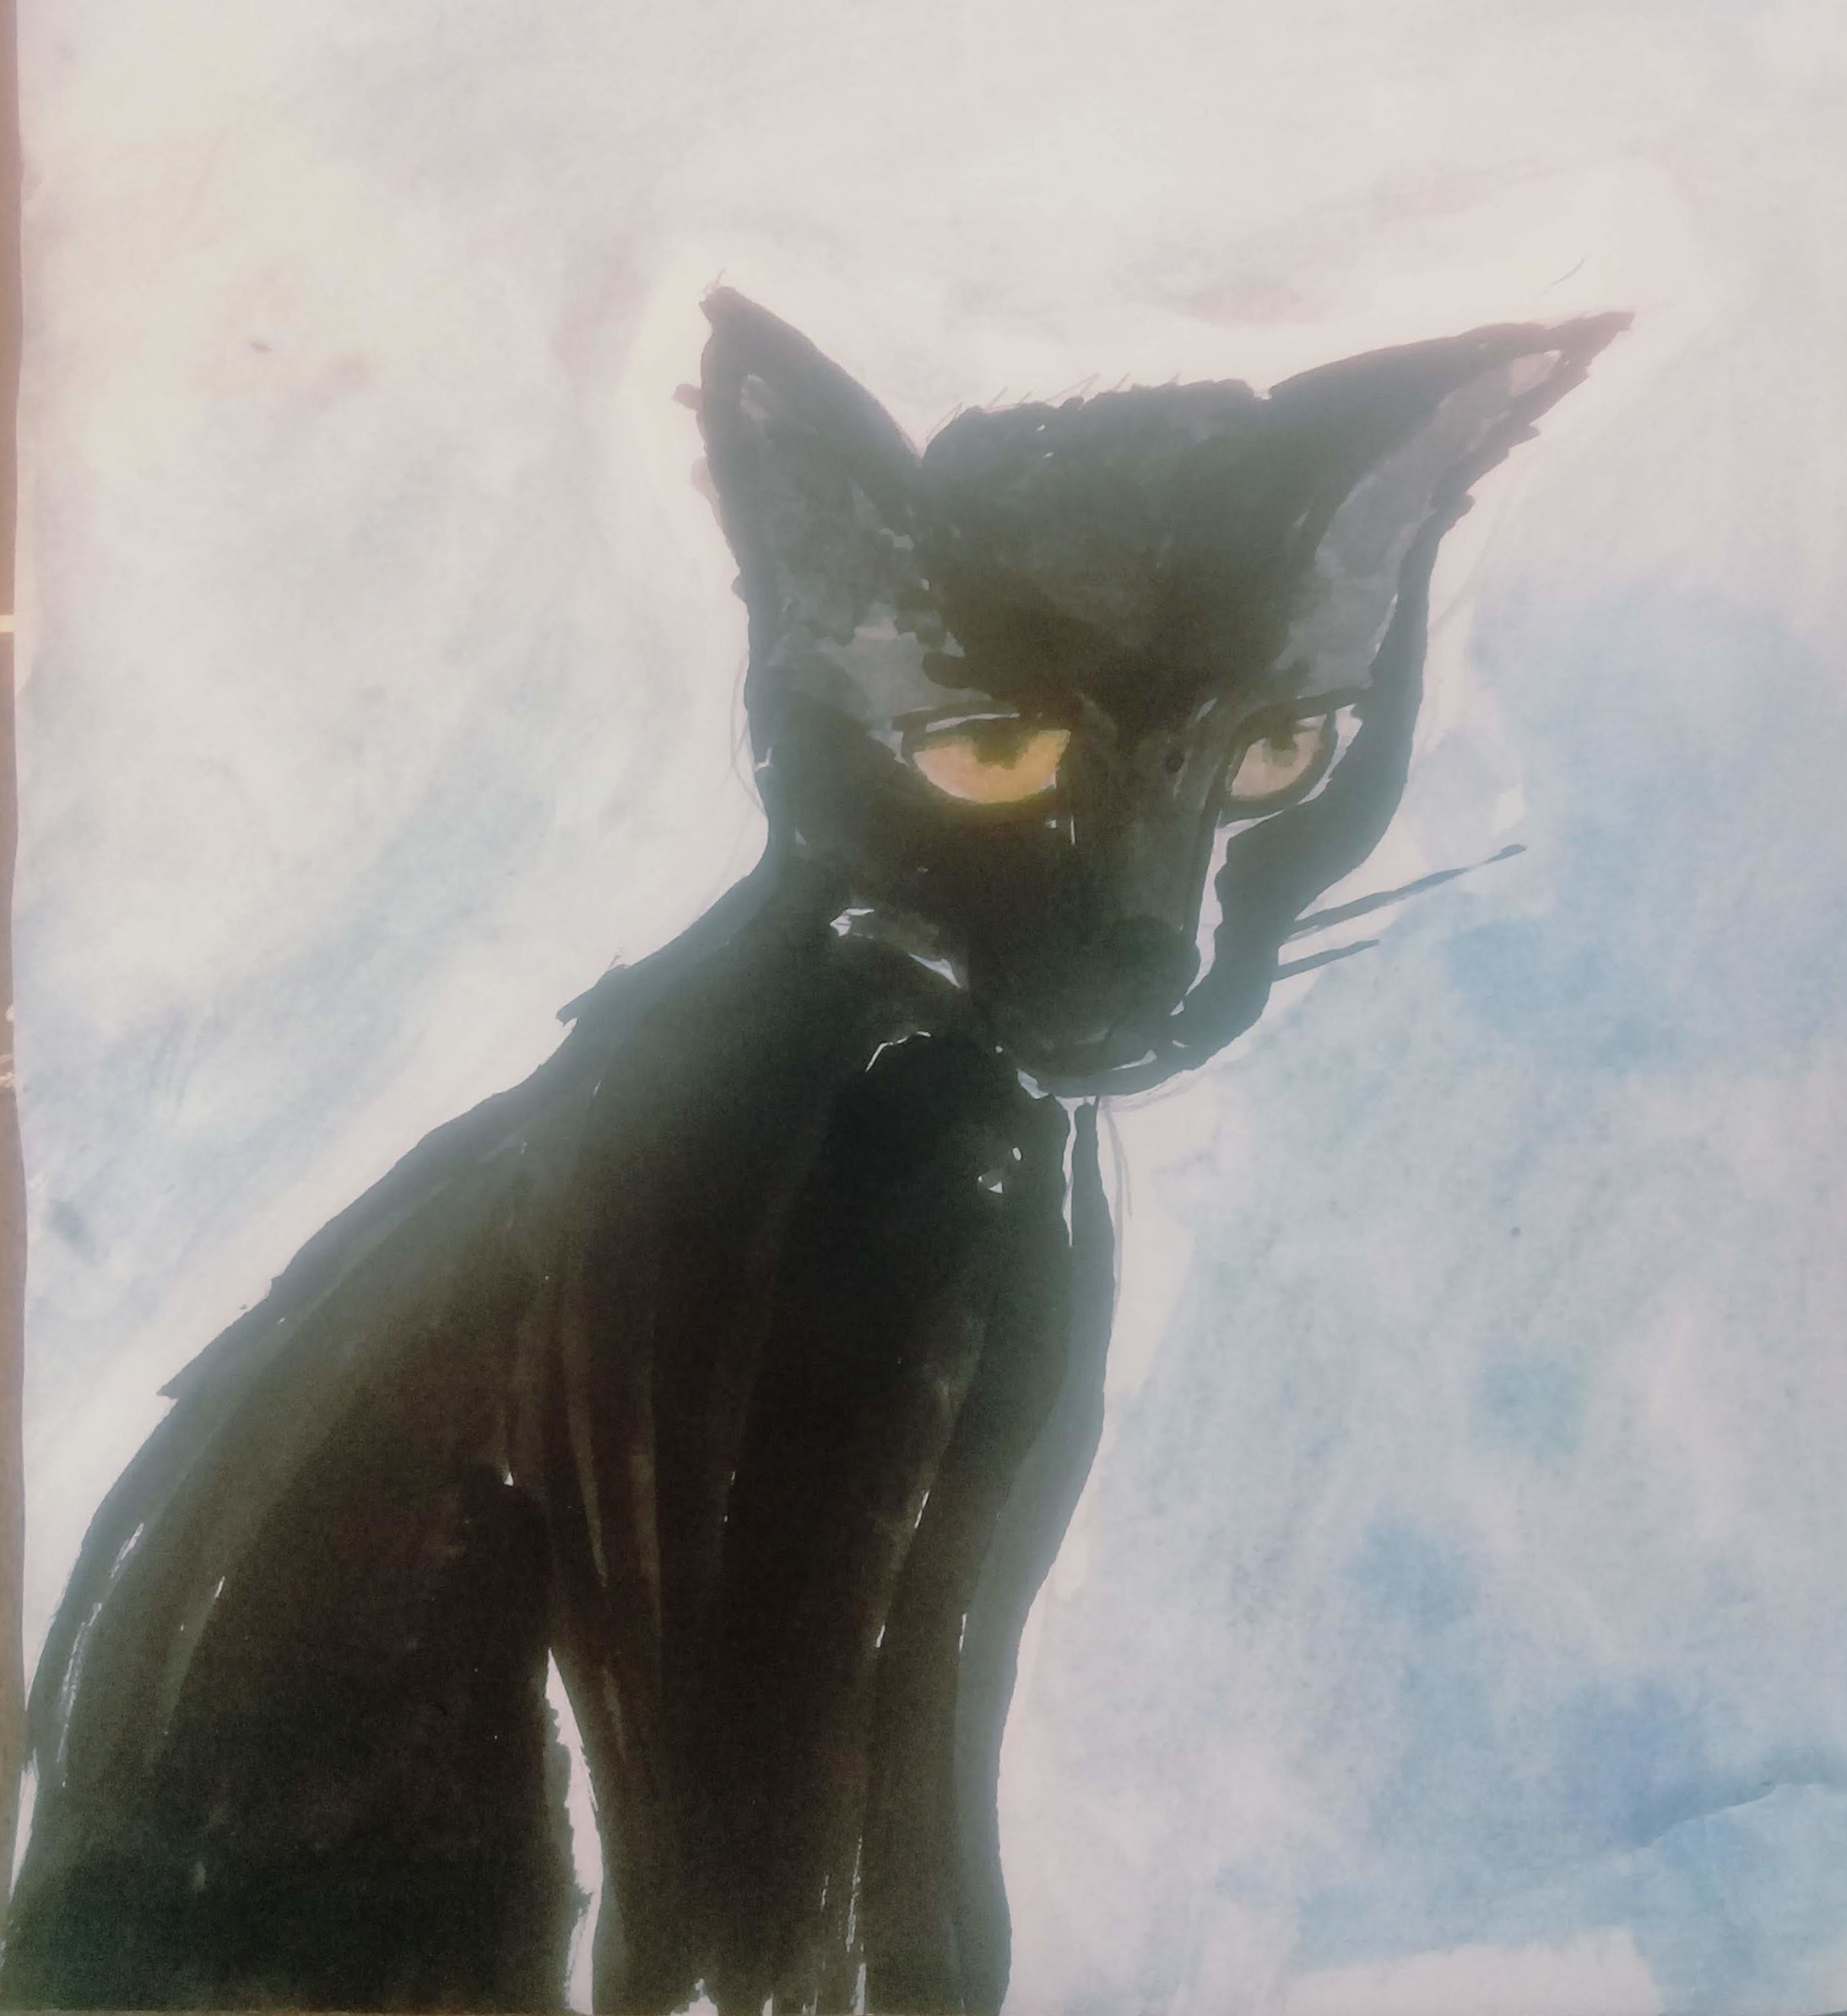
\includegraphics[width=.5\paperwidth ,angle=0]{reflexivo2}};	
	\node[text width=.45\paperwidth,xshift=-.2\paperwidth,yshift=0cm,scale=1] at (current page.center){
		NO, NO HABLO DE LAS PRODUCTORAS DE MIEL, NI DE LOS ZÁNGANOS O ABEJORROS. TAMPOCO DE LAS AVISPAS NI DE LOS TÁBANOS NI DE LAS POLILLAS. TODAS SON RESPETABLES CRIATURAS A LAS QUE PODRÍA ENFRENTARME Y CONVIVIR PERO EN ESTE CASO, QUERÍA HABLAR DEL ZUMBIDO BIEN CHILLÓN QUE TRAEN ¡LAS MOSCAS!
		
		ES HORA DE UN ANÁLISIS MÁS PROFUNDO.	};
	
	
	
	
\end{tikzpicture}
\newpage
\begin{tikzpicture}[remember picture, overlay]
	\node [inner sep=0pt, minimum width=\paperwidth, minimum height=\paperheight,opacity=1] at (current page.center) {
\includegraphics[width=\paperwidth,height=\paperheight,angle=0]{paper6}};
	
\end{tikzpicture} 


PUES PARA PODER CAZAR CORRECTAMENTE ES NECESARIO CONOCER A NUESTRAS PRESAS, LOS FELINOS LO TENEMOS MUY CLARO. PUEDEN OBSERVARNOS INMÓVILES DURANTE RATOS PROLONGADOS Y LO QUE HACEMOS ES APRENDER COMO SON LOS OTROS ANIMALES. Y LAS MOSCAS SI BIEN DESAGRADAN A LOS HUMANOS, CON SU ZUMBIDO MOLESTO, A LOS GATOS NOS DAN BUENA DIVERSIÓN. 

SEGURO SABEN DE LO RÁPIDAS QUE SON, SI PROBARON GOLPEARLAS, APUESTO A QUE VIERON QUE ESCAPAN CON FACILIDAD SI NO LO HACEN CON CUIDADO. POSEEN MUCHA SENSIBILIDAD A LAS MÍNIMAS CORRIENTES DE VIENTO QUE PUEDEN HACER CON SUS MANOS O CON OBJETOS. POR ESO YO ME ACERCO CON SIGILO.	 





\newpage
\begin{tikzpicture}[remember picture, overlay]
	\node [inner sep=0pt, minimum width=\paperwidth, minimum height=\paperheight,opacity=1] at (current page.center) {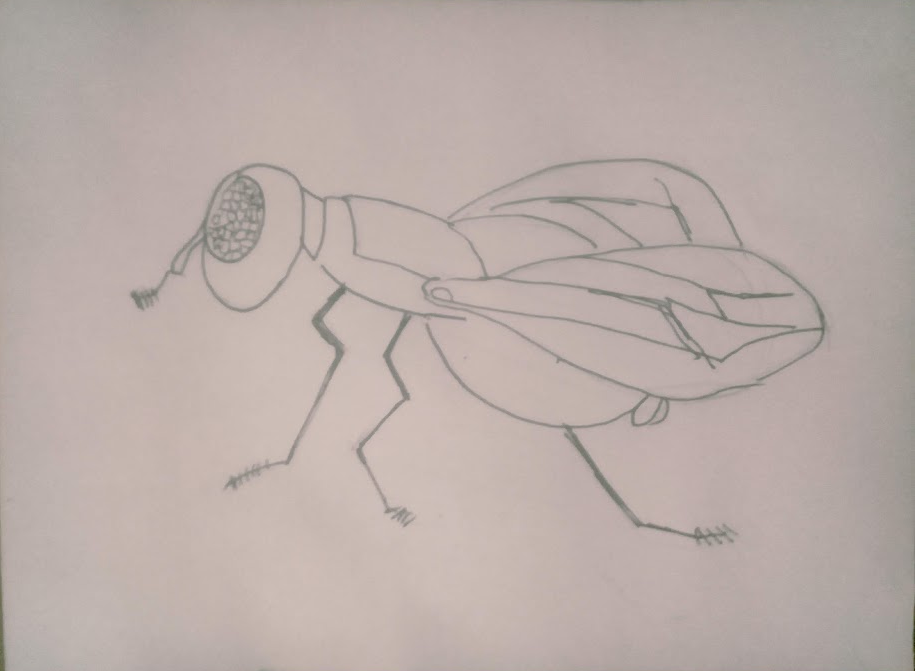
\includegraphics[width=\paperwidth,height=\paperheight,angle=0]{mosca1}};
	
\end{tikzpicture}
\newpage
\begin{tikzpicture}[remember picture, overlay]
	\node [inner sep=0pt, minimum width=\paperwidth, minimum height=\paperheight,opacity=1] at (current page.center) {
\includegraphics[width=\paperwidth,height=\paperheight,angle=0]{paper3}};
\end{tikzpicture}

UNA VEZ QUE UN GATO SE ENCUENTRA A UNA DISTANCIA DE UNA DE SUS PATAS DE UNA MOSCA, ES CASI SEGURO QUE VA A LOGRAR CAZARLA. TENEMOS MÁS RÁPIDOS REFLEJOS QUE LOS HUMANOS Y NUESTRAS FILOSAS GARRITAS SON MUY EFICACES. 

POR ESO, ME GUSTA CUANDO LAS VENTANAS ESTÁN ABIERTAS Y LAS MOSCAS PUEDEN ENTRAR A LA CASA. AUNQUE MI PADRE SIEMPRE TERMINA CERRANDO PARA QUE NO ENTREN LOS BICHOS$\ldots$ TAL VEZ NO SE DA CUENTA DE QUE NO HAY NADIE COMO UN BUEN GATO PARA CONTROLAR LOS BICHOS EN UNA CASA. SI A USTEDES LES MOLESTAN POR EJEMPLO LOS INSECTOS VOLADORES, BUSQUEN ESTAR AL LADO DE UN CONFIABLE FELINO Y ESTARÁN BIEN TRANQUILOS.	 
